% Dạng: test

% Dạng: test
\cauTN[id=C4-B11-D03-TH-007,muc=TH,loigiai={Ta có $\left(\sin\dfrac{x}{2}-\cos\dfrac{x}{2}\right)^2=1-\sin x$ nên $f(x)=1-\sin x+3x$, do đó $\displaystyle\int f(x)\,\mathrm{d}x=x+\cos x+\dfrac{3x^{2}}{2}+C$.}]{Họ tất cả các nguyên hàm của hàm số $f(x)=\left(\sin\dfrac{x}{2}-\cos\dfrac{x}{2}\right)^2+3x$ là}
  {$x+\cos x+\dfrac{3x^{2}}{2}+C$}
  {$x-\cos x+\dfrac{3x^{2}}{2}+C$}{$x+\cos x+3x^{2}+C$}{$-x+\cos x+\dfrac{3x^{2}}{2}+C$}


\cauTN[id=C4-B11-D03-VD-002,muc=VD,loigiai={Biến đổi $\dfrac{\cos 2x}{\sin^2x\cos^2x}=\dfrac{\cos^2x-\sin^2x}{\sin^2x\cos^2x}=\dfrac{1}{\sin^2x}-\dfrac{1}{\cos^2x}$, do đó $\displaystyle\int f(x)\,\mathrm{d}x=-\cot x-\tan x+C$.}]{Họ tất cả các nguyên hàm của hàm số $f(x)=\dfrac{\cos 2x}{\sin^2x\cos^2x}$ trên khoảng $\left(0;\dfrac{\pi}{2}\right)$ là}
  {$-\cot x-\tan x+C$}
  {$-\cot x+\tan x+C$}{$\cot x-\tan x+C$}{$\cot x+\tan x+C$}


\cauTLN[id=C4-B11-D03-NB-060,muc=NB,loigiai={$F(x)=-3\sin x-4\cos x+C$. $F\left(\frac{\pi}{2}\right)-F(0)=(-3+C)-(-4+C)=1$.}]{Cho $F(x)$ là một nguyên hàm của hàm số $f(x)=-3\cos x+4\sin x$. Tính $F\left(\dfrac{\pi}{2}\right)-F(0)$.}{1}


\cauTLN[id=C4-B11-D03-NB-050,muc=NB,loigiai={$F(x)=4\sin x-4\cos x+C$. $F\left(\frac{\pi}{2}\right)-F(0)=(4+C)-(-4+C)=8$.}]{Cho $F(x)$ là một nguyên hàm của hàm số $f(x)=4\cos x+4\sin x$. Tính $F\left(\dfrac{\pi}{2}\right)-F(0)$.}{8}


% Dạng: test
\cauDS[id=C5-B14-D02-VD-044,muc=VD,loigiai={$\vec n_R=\left[\vec n_P,\vec n_Q\right]=(4;2;3)$, $(R)\colon 4x+2y+3z+3=0$. a) Đúng. b) Sai: vì $3\ne0$. c) Sai: vectơ đó không vuông góc với $\vec n_P$. d) Đúng.}]{Trong không gian $Oxyz$, cho hai mặt phẳng $(P)\colon x-2y-7=0$, $(Q)\colon 3y-2z-6=0$ và mặt phẳng $(R)$ đi qua $M(0;-3;1)$, vuông góc với cả $(P)$ và $(Q)$. Xét tính đúng sai của các mệnh đề sau:}{%
  \y{Phương trình của $(R)$ là $4x+2y+3z+3=0$.}{d}
  \y{$(R)$ đi qua gốc toạ độ.}{s}
  \y{$(R)$ nhận $\vec n_P+\vec n_Q=(1;1;-2)$ làm một vectơ pháp tuyến.}{s}
  \y{$(R)$ nhận $\left[\vec n_P,\vec n_Q\right]=(4;2;3)$ làm một vectơ pháp tuyến.}{d}}


\cauDS[id=C5-B14-D02-TH-061,muc=TH,loigiai={$\overrightarrow{AB}=(-4;0;3)$, $\overrightarrow{AC}=(1;2;-2)$, $\left[\overrightarrow{AB},\overrightarrow{AC}\right]=(-6;-5;-8)$, $(ABC)\colon 6x+5y+8z-10=0$. a) Sai: thay vào được $-12\ne0$. b) Đúng. c) Sai: đúng là $6x+5y+8z-10=0$. d) Sai: thay $O$ vào được $-10\ne 0$.}]{Trong không gian $Oxyz$, cho ba điểm $A(0;2;0)$, $B(-4;2;3)$, $C(1;4;-2)$. Xét tính đúng sai của các mệnh đề sau:}{%
  \y{Điểm $D(3;-4;0)$ thuộc mặt phẳng $(ABC)$.}{s}
  \y{Mặt phẳng $(ABC)$ có phương trình $6x+5y+8z-10=0$.}{d}
  \y{Mặt phẳng $(ABC)$ có phương trình $6x+5y+8z+10=0$.}{s}
  \y{Mặt phẳng $(ABC)$ đi qua gốc toạ độ.}{s}}


\cauTLN[id=C5-B14-D02-TH-079,muc=TH,loigiai={Trung điểm $I(2;\dfrac{5}{2};-\dfrac{1}{2})$, $\overrightarrow{AB}=(2;-3;-3)$; mặt phẳng trung trực: $2x-3y-3z+2=0$. Chia cho $2$: $b+c+d=-2$.}]{Trong không gian $Oxyz$, mặt phẳng trung trực của đoạn thẳng $AB$ với $A(1;4;1)$, $B(3;1;-2)$ có phương trình dạng $x+by+cz+d=0$. Tính $b+c+d$.}{-2}


\cauTN[id=C5-B14-D02-VD-001,muc=VD,loigiai={$\vec n_P=\left[\overrightarrow{AB},\vec n_Q\right]=(-3;3;3)$; $(P)\colon x-y-z-2=0$.}]{Trong không gian $Oxyz$, phương trình của mặt phẳng $(P)$ đi qua hai điểm $A(1;-2;1)$, $B(4;2;0)$ và vuông góc với mặt phẳng $(Q)\colon y-z+7=0$ là}
  {$x-y-z-2=0$}
  {$y-z+3=0$}{$x+y-z+2=0$}{$x-y-z+2=0$}


% Dạng: test
\cauTN[id=T11-C7-B23-D29-VD-122,muc=VD,loigiai={Cột vuông góc với mặt sân nên vuông góc với đường nối chân cột và móc neo; $L=\sqrt{15^2+8^2}\approx17$ m.}]{Để cột ăng-ten cao $15$ m trên sân thượng trường đứng vững trước gió mùa, người ta căng các dây cáp từ đỉnh cột xuống các móc neo trên mặt sân thượng; mỗi móc neo cách chân cột $8$ m. Cột được dựng vuông góc với mặt sân thượng. Mỗi sợi dây cáp dài bao nhiêu mét (coi dây căng thẳng, làm tròn đến hàng phần mười)?}
  {$17$.}
  {$19$.}{$15$.}{$14$.}


\cauTLN[id=T11-C7-B23-D29-TH-102,muc=TH,loigiai={Cột vuông góc với mặt sân nên vuông góc với đường nối chân cột và móc neo; $L=\sqrt{10^2+6^2}\approx11{,}7$ m.}]{Để cột ăng-ten cao $10$ m trên sân thượng trường đứng vững trước gió mùa, người ta căng các dây cáp từ đỉnh cột xuống các móc neo trên mặt sân thượng; mỗi móc neo cách chân cột $6$ m. Cột được dựng vuông góc với mặt sân thượng. Mỗi sợi dây cáp dài bao nhiêu mét (coi dây căng thẳng, làm tròn đến hàng phần mười)?}{11,7}


\cauTLN[id=T11-C7-B23-D29-NB-039,muc=NB,loigiai={Các đường thẳng vuông góc với $(ADB')$: không có.}]{Cho hình lập phương $ABCD.A'B'C'D'$ có cạnh bằng $a$. Trong các đường thẳng chứa cạnh của khối đã cho, có bao nhiêu đường thẳng vuông góc với mặt phẳng $(ADB')$?\begin{center}
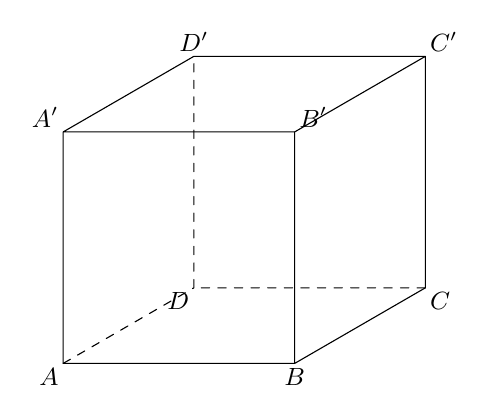
\begin{tikzpicture}[line join=round,line cap=round,font=\small]
\draw[dashed] (4.60,0.96)--(1.66,0.96) (0.00,0.00)--(1.66,0.96) (1.66,0.96)--(1.66,3.90);
\draw (0.00,0.00)--(2.94,0.00) (2.94,0.00)--(4.60,0.96) (0.00,2.94)--(2.94,2.94) (2.94,2.94)--(4.60,3.90) (4.60,3.90)--(1.66,3.90) (0.00,2.94)--(1.66,3.90) (2.94,0.00)--(2.94,2.94) (0.00,0.00)--(0.00,2.94) (4.60,0.96)--(4.60,3.90);
\node[anchor=north east,inner sep=1.5pt] at (0.00,0.00) {$A$};
\node[anchor=north,inner sep=1.5pt] at (2.94,0.00) {$B$};
\node[anchor=north west,inner sep=1.5pt] at (4.60,0.96) {$C$};
\node[anchor=north east,inner sep=1.5pt] at (1.66,0.96) {$D$};
\node[anchor=south east,inner sep=1.5pt] at (0.00,2.94) {$A'$};
\node[anchor=south west,inner sep=1.5pt] at (2.94,2.94) {$B'$};
\node[anchor=south west,inner sep=1.5pt] at (4.60,3.90) {$C'$};
\node[anchor=south,inner sep=1.5pt] at (1.66,3.90) {$D'$};
\end{tikzpicture}
\end{center}}{0}


\cauTN[id=T11-C7-B23-D29-TH-060,muc=TH,loigiai={$CD$ vuông góc với hai đường thẳng cắt nhau nằm trong $(SAD)$ nên $CD\perp(SAD)$.}]{Cho hình chóp $S.ABCD$ có đáy là hình vuông $ABCD$ cạnh $a$, $SA$ vuông góc với mặt phẳng đáy và $SA=\dfrac{a\sqrt{2}}{2}$. Đường thẳng $CD$ vuông góc với mặt phẳng nào sau đây?\begin{center}
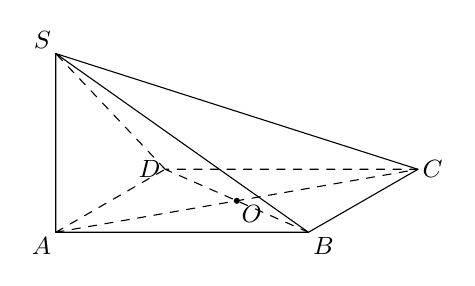
\begin{tikzpicture}[line join=round,line cap=round,font=\small]
\draw[dashed] (4.60,0.80)--(1.39,0.80) (0.00,0.00)--(1.39,0.80) (1.39,0.80)--(0.00,2.27) (0.00,0.00)--(4.60,0.80) (3.21,0.00)--(1.39,0.80);
\draw (0.00,0.00)--(3.21,0.00) (3.21,0.00)--(4.60,0.80) (0.00,0.00)--(0.00,2.27) (3.21,0.00)--(0.00,2.27) (4.60,0.80)--(0.00,2.27);
\node[anchor=north east,inner sep=1.5pt] at (0.00,0.00) {$A$};
\node[anchor=north west,inner sep=1.5pt] at (3.21,0.00) {$B$};
\node[anchor=west,inner sep=1.5pt] at (4.60,0.80) {$C$};
\node[anchor=east,inner sep=1.5pt] at (1.39,0.80) {$D$};
\node[anchor=south east,inner sep=1.5pt] at (0.00,2.27) {$S$};
\fill (2.30,0.40) circle (1.1pt);
\node[anchor=north west,inner sep=1.5pt] at (2.30,0.40) {$O$};
\end{tikzpicture}
\end{center}}
  {$(SAD)$.}
  {$(SAB)$.}{$(SBD)$.}{$(SAC)$.}


\cauTN[id=T11-C7-B23-D29-TH-046,muc=TH,loigiai={$AC$ vuông góc với hai đường thẳng cắt nhau nằm trong $(SBD)$ nên $AC\perp(SBD)$.}]{Cho hình chóp tứ giác đều $S.ABCD$ có cạnh đáy bằng $a$, cạnh bên bằng $\dfrac{a\sqrt{5}}{2}$ và $O$ là tâm của đáy. Đường thẳng $AC$ vuông góc với mặt phẳng nào sau đây?\begin{center}
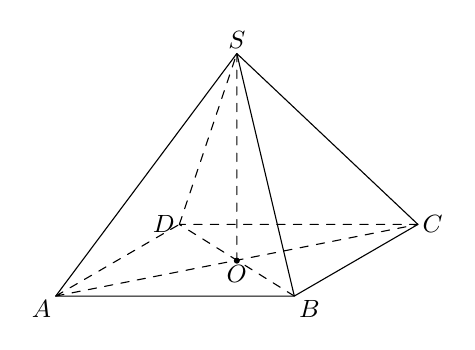
\begin{tikzpicture}[line join=round,line cap=round,font=\small]
\draw[dashed] (4.60,0.91)--(1.57,0.91) (0.00,0.00)--(1.57,0.91) (1.57,0.91)--(2.30,3.08) (0.00,0.00)--(4.60,0.91) (3.03,0.00)--(1.57,0.91) (2.30,3.08)--(2.30,0.45);
\draw (0.00,0.00)--(3.03,0.00) (3.03,0.00)--(4.60,0.91) (0.00,0.00)--(2.30,3.08) (3.03,0.00)--(2.30,3.08) (4.60,0.91)--(2.30,3.08);
\node[anchor=north east,inner sep=1.5pt] at (0.00,0.00) {$A$};
\node[anchor=north west,inner sep=1.5pt] at (3.03,0.00) {$B$};
\node[anchor=west,inner sep=1.5pt] at (4.60,0.91) {$C$};
\node[anchor=east,inner sep=1.5pt] at (1.57,0.91) {$D$};
\node[anchor=south,inner sep=1.5pt] at (2.30,3.08) {$S$};
\fill (2.30,0.45) circle (1.1pt);
\node[anchor=north,inner sep=1.5pt] at (2.30,0.45) {$O$};
\end{tikzpicture}
\end{center}}
  {$(SBD)$.}
  {$(SAB)$.}{$(SCD)$.}{$(SBC)$.}


\cauTN[id=T11-C7-B23-D29-VDC-136,muc=VDC,loigiai={$AD$ vuông góc với hai đường thẳng cắt nhau nằm trong $(SAB)$ nên $AD\perp(SAB)$.}]{Một chiếc lều cắm trại dã ngoại của lớp 11A2 được dựng trên nền đất phẳng. Mô hình hoá bằng hình chóp $S.ABCD$ có đáy là hình vuông cạnh $a$, tam giác $SAB$ đều và nằm trong mặt phẳng vuông góc với mặt phẳng đáy; gọi $H$ là trung điểm của $AB$. Đường thẳng $AD$ vuông góc với mặt phẳng nào sau đây?\begin{center}
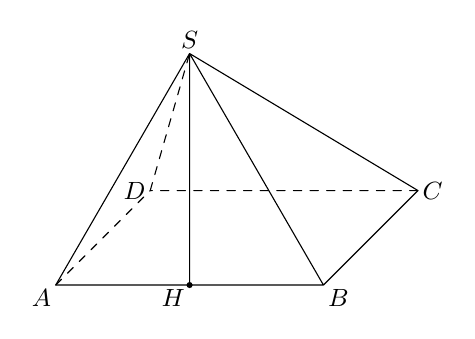
\begin{tikzpicture}[line join=round,line cap=round,font=\small]
\draw[dashed] (4.60,1.20)--(1.20,1.20) (0.00,0.00)--(1.20,1.20) (1.20,1.20)--(1.70,2.94);
\draw (0.00,0.00)--(3.40,0.00) (3.40,0.00)--(4.60,1.20) (0.00,0.00)--(1.70,2.94) (3.40,0.00)--(1.70,2.94) (4.60,1.20)--(1.70,2.94) (1.70,2.94)--(1.70,0.00);
\node[anchor=north east,inner sep=1.5pt] at (0.00,0.00) {$A$};
\node[anchor=north west,inner sep=1.5pt] at (3.40,0.00) {$B$};
\node[anchor=west,inner sep=1.5pt] at (4.60,1.20) {$C$};
\node[anchor=east,inner sep=1.5pt] at (1.20,1.20) {$D$};
\node[anchor=south,inner sep=1.5pt] at (1.70,2.94) {$S$};
\fill (1.70,0.00) circle (1.1pt);
\node[anchor=north east,inner sep=1.5pt] at (1.70,0.00) {$H$};
\end{tikzpicture}
\end{center}}
  {$(SAB)$.}
  {$(SAC)$.}{$(SBD)$.}{$(SCD)$.}


% Dạng: test
\cauTN[id=C1-B5-D01-TH-040,muc=TH,loigiai={Vận tốc $v(t)=x'(t)=-3 \pi\sin(\pi t)$ (cm/s), gia tốc $a(t)=v'(t)=-3 \pi^{2}\cos(\pi t)$ (cm/s$^2$). $v(\dfrac{1}{3})=- \dfrac{3 \sqrt{3} \pi}{2}$.}]{Một vật dao động điều hòa có phương trình li độ $x(t)=3\cos(\pi t)$ (cm), với $t$ tính bằng giây. Vận tốc của vật tại thời điểm $t=\dfrac{1}{3}$ giây bằng}
  {$- \dfrac{3 \sqrt{3} \pi}{2}\,\mathrm{cm/s}$.}
  {$- \dfrac{3 \sqrt{3} \pi}{4}\,\mathrm{cm/s}$.}{$- \dfrac{9 \sqrt{3} \pi}{4}\,\mathrm{cm/s}$.}{$- \dfrac{3 \sqrt{3} \pi}{2} + 1\,\mathrm{cm/s}$.}


\cauTLN[id=C1-B5-D01-VD-050,muc=VD,loigiai={Ta có $x(\dfrac{1}{2})=6$. Kết quả: $6$.}]{Một vật dao động điều hòa có phương trình li độ $x(t)=6\cos(4 \pi t)$ (cm), với $t$ tính bằng giây. Tìm li độ của vật tại thời điểm $t=\dfrac{1}{2}$ giây (đơn vị: $\mathrm{cm}$).}{6}


\cauTN[id=C1-B5-D01-NB-004,muc=NB,loigiai={Ta có $h(\dfrac{1}{2})=\dfrac{65}{4}$.}]{Một quả bóng được ném thẳng đứng lên trên từ độ cao $5$ m với vận tốc ban đầu $25$ m/s. Độ cao của quả bóng (tính bằng mét) sau $t$ giây là $h(t)=5+25t-5t^2$ (bỏ qua sức cản không khí, lấy $g=10$ m/s$^2$). Độ cao của quả bóng tại thời điểm $t=\dfrac{1}{2}$ giây bằng}
  {$\dfrac{65}{4}\,\mathrm{m}$.}
  {$\dfrac{4}{65}\,\mathrm{m}$.}{$65\,\mathrm{m}$.}{$\dfrac{61}{4}\,\mathrm{m}$.}


\cauTN[id=C1-B5-D01-VD-032,muc=VD,loigiai={Vận tốc $v(t)=x'(t)=-5 \pi\sin(\pi t)$ (cm/s), gia tốc $a(t)=v'(t)=-5 \pi^{2}\cos(\pi t)$ (cm/s$^2$). $v(\dfrac{1}{6})=- \dfrac{5 \pi}{2}$.}]{Một vật dao động điều hòa có phương trình li độ $x(t)=5\cos(\pi t)$ (cm), với $t$ tính bằng giây. Vận tốc của vật tại thời điểm $t=\dfrac{1}{6}$ giây bằng}
  {$- \dfrac{5 \pi}{2}\,\mathrm{cm/s}$.}
  {$- \dfrac{5 \pi}{2} - 1\,\mathrm{cm/s}$.}{$- \dfrac{5 \pi}{3}\,\mathrm{cm/s}$.}{$- \dfrac{5 \pi}{4}\,\mathrm{cm/s}$.}


% Dạng: test
\cauTLN[id=C4-B11-D02-VD-059,muc=VD,loigiai={$f(x)=x^{2}+6+\dfrac{9}{x^2}$, $F(x)=\dfrac{x^{3}}{3}+6x-\dfrac{9}{x}$, $F(3)-F(1)=\dfrac{80}{3}$.}]{Cho $F(x)$ là một nguyên hàm của $f(x)=\left(- x-\dfrac{3}{x}\right)^2$ trên $(0;+\infty)$. Tính $F(3)-F(1)$ (làm tròn kết quả đến hàng phần mười).}{26,7}


\cauTN[id=C4-B11-D02-NB-017,muc=NB,loigiai={Theo bảng nguyên hàm và tính chất của nguyên hàm: $\displaystyle\int\left(4x-2\right)\mathrm{d}x=2x^{2}-2x+C$.}]{Họ tất cả các nguyên hàm của hàm số $f(x)=4x-2$ là}
  {$2x^{2}-2x+C$}
  {$2x^{2}+2x+C$}{$8x^{2}-2x+C$}{$2x^{2}-2+C$}


\cauDS[id=C4-B11-D02-NB-041,muc=NB,loigiai={Theo bảng nguyên hàm và tính chất của nguyên hàm: $\displaystyle\int\left(-3x^{2}-8x+4\right)\mathrm{d}x=-x^{3}-4x^{2}+4x+C$. a) Sai: đúng là $-\dfrac1x+C$. b) Đúng. c) Đúng. d) Sai.}]{Cho hàm số $f(x)=-3x^{2}-8x+4$. Xét tính đúng sai của các mệnh đề sau:}{%
  \y{$\displaystyle\int \dfrac{1}{x^2}\,\mathrm{d}x=\dfrac{1}{x}+C$ trên mỗi khoảng xác định.}{s}
  \y{$\displaystyle\int f(x)\,\mathrm{d}x=-x^{3}-4x^{2}+4x+C$.}{d}
  \y{$\displaystyle\int \dfrac{1}{x}\,\mathrm{d}x=\ln|x|+C$ trên mỗi khoảng xác định.}{d}
  \y{$\displaystyle\int f(x)\,\mathrm{d}x=-9x^{3}-16x^{2}+4x+C$.}{s}}


\cauTLN[id=C4-B11-D02-VD-055,muc=VD,loigiai={$f(x)=1+\dfrac{4}{\sqrt{x}}+\dfrac{4}{x}$, $F(x)=x+8\sqrt{x}+4\ln|x|$. $F(4)-F(1)=11+4\ln 4$ nên $p=11$.}]{Cho $F(x)$ là một nguyên hàm của $f(x)=\dfrac{(\sqrt{x}+2)^2}{x}$ trên $(0;+\infty)$. Biết $F(4)-F(1)=p+q\ln 4$ với $p$, $q$ là các số hữu tỉ. Tính $p$.}{11}


% Dạng: test
\cauTN[id=C2-B6-D03-VD-012,muc=VD,loigiai={Ta có $\overrightarrow{GF}\cdot \overrightarrow{DB}=9$, $|\overrightarrow{GF}|^2=9$, $|\overrightarrow{DB}|^2=18$ nên $\cos(\overrightarrow{GF},\overrightarrow{DB})=\dfrac{\sqrt{2}}{2}$.}]{Cho hình lập phương $ABCD.EFGH$ có cạnh bằng $3$. Giá trị $\cos(\overrightarrow{GF},\overrightarrow{DB})$ bằng}
  {$\dfrac{\sqrt{2}}{2}$.}
  {$\dfrac{5\sqrt{2}}{9}$.}{$-\dfrac{\sqrt{2}}{2}$.}{$\dfrac{4\sqrt{2}}{9}$.}


\cauTN[id=C2-B6-D03-NB-011,muc=NB,loigiai={Biểu diễn hai vectơ theo ba cạnh xuất phát từ một đỉnh: $\overrightarrow{SA}=\vec{a}$, $\overrightarrow{SC}=\vec{c}$, rồi dùng $\vec{x}\cdot\vec{y}$ theo các tích vô hướng cơ bản ta được $\dfrac{9}{2}$.}]{Cho tứ diện đều $SABC$ có cạnh bằng $3$. Tích vô hướng $\overrightarrow{SA}\cdot \overrightarrow{SC}$ bằng}
  {$\dfrac{9}{2}$.}
  {$\dfrac{11}{2}$.}{$\dfrac{7}{2}$.}{$-\dfrac{9}{2}$.}


\cauTN[id=C2-B6-D03-TH-018,muc=TH,loigiai={Ta có $\overrightarrow{AF}\cdot \overrightarrow{EB}=0$, $|\overrightarrow{AF}|^2=18$, $|\overrightarrow{EB}|^2=18$ nên $\cos=\dfrac{0}{\sqrt{18\cdot 18}}$, suy ra góc bằng $90^\circ$.}]{Cho hình lập phương $ABCD.EFGH$ có cạnh bằng $3$. Góc giữa hai vectơ $\overrightarrow{AF}$ và $\overrightarrow{EB}$ bằng}
  {$90^\circ$.}
  {$150^\circ$.}{$120^\circ$.}{$45^\circ$.}


\cauTLN[id=C2-B6-D03-VD-060,muc=VD,loigiai={Phân tích theo ba cạnh xuất phát từ một đỉnh ta được tích vô hướng bằng $0$.}]{Cho hình hộp chữ nhật $ABCD.A'B'C'D'$ có $AB=3$, $AD=2$, $AA'=3$. Tính $\overrightarrow{BA'}\cdot \overrightarrow{AC'}$.}{0}

% Dạng: test
\cauTN[id=C4-B13-D01-NB-008,muc=NB,loigiai={$S=\displaystyle\int_{0}^{1}\left|x^{2} + 2\right|\,\mathrm{d}x=\dfrac{7}{3}$.}]{Diện tích hình phẳng giới hạn bởi đồ thị hàm số $y=x^{2} + 2$, trục hoành và hai đường thẳng $x=0$, $x=1$ bằng}
  {$\dfrac{7}{3}$}
  {$\dfrac{7 \pi}{3}$}{$-\dfrac{7}{3}$}{$\dfrac{10}{3}$}


\cauTN[id=C4-B13-D01-TH-009,muc=TH,loigiai={$S=\displaystyle\int_{0}^{\ln 2}\left|\mathrm{e}^x\right|\,\mathrm{d}x=1$.}]{Diện tích hình phẳng giới hạn bởi đồ thị hàm số $y=\mathrm{e}^x$, trục hoành và hai đường thẳng $x=0$, $x=\ln 2$ bằng}
  {$1$}
  {$\pi$}{$\dfrac{1}{2}$}{$2$}


\cauDS[id=C4-B13-D01-TH-062,muc=TH,loigiai={$- x^{2} + x + 6=0$ có nghiệm $x=3$ trên $(-2;4)$. $S=\displaystyle\int_{-2}^{4}\left|- x^{2} + x + 6\right|\,\mathrm{d}x=\left|\displaystyle\int_{-2}^{3}(- x^{2} + x + 6)\,\mathrm{d}x\right|+\left|\displaystyle\int_{3}^{4}(- x^{2} + x + 6)\,\mathrm{d}x\right|=\dfrac{71}{3}$. a) Đúng. b) Đúng. c) Sai: hàm số đổi dấu trên đoạn. d) Đúng.}]{Gọi $S$ là diện tích hình phẳng giới hạn bởi đồ thị hàm số $y=- x^{2} + x + 6$, trục hoành và hai đường thẳng $x=-2$, $x=4$. Xét tính đúng sai của các mệnh đề sau:}{%
  \y{Phương trình $- x^{2} + x + 6=0$ có nghiệm $x=3$ thuộc khoảng $(-2;4)$.}{d}
  \y{$S=\displaystyle\int_{-2}^{4}\left|- x^{2} + x + 6\right|\,\mathrm{d}x$.}{d}
  \y{$S=\left|\displaystyle\int_{-2}^{4}(- x^{2} + x + 6)\,\mathrm{d}x\right|$.}{s}
  \y{$\displaystyle\int_{-2}^{4}(- x^{2} + x + 6)\,\mathrm{d}x=18$.}{d}}


\cauTN[id=C4-B13-D01-VD-013,muc=VD,loigiai={Phương trình $x^{3} - 2 x^{2} - 5 x + 6=0$ có các nghiệm $x=-2, 1, 3$. $S=\left|\displaystyle\int_{-2}^{1}(x^{3} - 2 x^{2} - 5 x + 6)\,\mathrm{d}x\right|+\left|\displaystyle\int_{1}^{3}(x^{3} - 2 x^{2} - 5 x + 6)\,\mathrm{d}x\right|=\dfrac{253}{12}$.}]{Diện tích hình phẳng giới hạn bởi đồ thị hàm số $y=x^{3} - 2 x^{2} - 5 x + 6$ và trục hoành bằng}
  {$\dfrac{253}{12}$}
  {$\dfrac{125}{12}$}{$-\dfrac{125}{12}$}{$\dfrac{253 \pi}{12}$}


% Dạng: test
\cauTLN[id=T11-C8-B28-D34-TH-100,muc=TH,loigiai={$n(A)=5$, $n(B)=6$, $n(A\cap B)=1$; $n(A\cup B)=5+6-1=10$.}]{Gieo một con xúc xắc cân đối hai lần liên tiếp. Gọi $A$ là biến cố "Tổng số chấm hai lần gieo bằng $6$" và $B$ là biến cố "Lần thứ nhất xuất hiện mặt $2$ chấm". Biến cố $A\cup B$ có bao nhiêu kết quả thuận lợi?}{10}


\cauTN[id=T11-C8-B28-D34-VD-110,muc=VD,loigiai={$P(A\cup B)=\dfrac{16+10-5}{45}=\dfrac{7}{15}$.}]{Lớp 11A1 trường THPT Trần Hưng Đạo có $45$ học sinh, trong đó có $16$ học sinh tham gia câu lạc bộ Bóng đá, $10$ học sinh tham gia câu lạc bộ Cờ vua và $5$ học sinh tham gia cả hai câu lạc bộ. Chọn ngẫu nhiên một học sinh của lớp. Gọi $A$ là biến cố "học sinh đó tham gia câu lạc bộ Bóng đá", $B$ là biến cố "học sinh đó tham gia câu lạc bộ Cờ vua". Xác suất của biến cố $A\cup B$ bằng}
  {$\dfrac{7}{15}$.}
  {$\dfrac{7}{30}$.}{$\dfrac{26}{45}$.}{$\dfrac{17}{30}$.}


\cauTLN[id=T11-C8-B28-D34-TH-102,muc=TH,loigiai={$n(A)=10$, $n(B)=5$, $n(A\cap B)=5$; $n(A\cup B)=10$.}]{Chọn ngẫu nhiên một số trong các số nguyên từ $1$ đến $30$. Gọi $A$: "Số được chọn chia hết cho $3$", $B$: "Số được chọn chia hết cho $6$". Biến cố $A\cup B$ có bao nhiêu kết quả thuận lợi?}{10}


\cauTLN[id=T11-C8-B28-D34-VDC-148,muc=VDC,loigiai={$P=\dfrac{(14-5)+(11-5)}{45}=\dfrac{1}{3}$.}]{Lớp 11A1 trường THPT Phan Bội Châu có $45$ học sinh, trong đó có $14$ học sinh tham gia câu lạc bộ Bóng đá, $11$ học sinh tham gia câu lạc bộ Cờ vua và $5$ học sinh tham gia cả hai câu lạc bộ. Chọn ngẫu nhiên một học sinh của lớp. Gọi $A$ là biến cố "học sinh đó tham gia câu lạc bộ Bóng đá", $B$ là biến cố "học sinh đó tham gia câu lạc bộ Cờ vua". Tính xác suất để học sinh được chọn tham gia đúng một trong hai câu lạc bộ (làm tròn đến hàng phần trăm).}{0,33}


% Dạng: test
\cauDS[id=C4-B12-D01-TH-054,muc=TH,loigiai={Áp dụng tính chất tuyến tính và tính chất đổi cận của tích phân; $\displaystyle\int_{1}^{3}x\,\mathrm{d}x=4$. a) Sai. b) Sai: đúng là $13$. c) Đúng. d) Sai: không có tính chất tích phân của tích.}]{Cho các hàm số $f(x)$, $g(x)$ liên tục trên $\mathbb{R}$ thoả mãn $\displaystyle\int_{1}^{3}f(x)\,\mathrm{d}x=9$ và $\displaystyle\int_{1}^{3}g(x)\,\mathrm{d}x=-7$. Xét tính đúng sai của các mệnh đề sau:}{%
  \y{$\displaystyle\int_{1}^{3}\left[-f(x)+3g(x)\right]\,\mathrm{d}x=12$.}{s}
  \y{$\displaystyle\int_{1}^{3}\left[f(x)+x\right]\,\mathrm{d}x=11$.}{s}
  \y{$\displaystyle\int_{1}^{3}\left[-f(x)+3g(x)\right]\,\mathrm{d}x=-30$.}{d}
  \y{$\displaystyle\int_{1}^{3}f(x)g(x)\,\mathrm{d}x=-63$.}{s}}


\cauTN[id=C4-B12-D01-NB-035,muc=NB,loigiai={$\displaystyle\int_{2}^{-2}f(x)\,\mathrm{d}x=-\displaystyle\int_{-2}^{2}f(x)\,\mathrm{d}x=-1$.}]{Biết $\displaystyle\int_{-2}^{2}f(x)\,\mathrm{d}x=1$. Giá trị của $\displaystyle\int_{2}^{-2}f(x)\,\mathrm{d}x$ bằng}
  {$-1$}
  {$1$}{$0$}{$2$}


\cauTN[id=C4-B12-D01-TH-034,muc=TH,loigiai={$\displaystyle\int_{1}^{3}\left[2f(x)-2x+1\right]\,\mathrm{d}x=2\displaystyle\int_{1}^{3}f(x)\,\mathrm{d}x+\displaystyle\int_{1}^{3}(-2x+1)\,\mathrm{d}x=2\cdot(2)+-6=-2$.}]{Biết $\displaystyle\int_{1}^{3}f(x)\,\mathrm{d}x=2$. Giá trị của $\displaystyle\int_{1}^{3}\left[2f(x)-2x+1\right]\,\mathrm{d}x$ bằng}
  {$-2$}
  {$-10$}{$3$}{$-4$}


\cauTN[id=C4-B12-D01-NB-025,muc=NB,loigiai={$\displaystyle\int_{1}^{2}\left[-f(x)-g(x)\right]\,\mathrm{d}x=-1\cdot \displaystyle\int_{1}^{2}f(x)\,\mathrm{d}x-1\cdot \displaystyle\int_{1}^{2}g(x)\,\mathrm{d}x=2$.}]{Biết $\displaystyle\int_{1}^{2}f(x)\,\mathrm{d}x=-1$ và $\displaystyle\int_{1}^{2}g(x)\,\mathrm{d}x=-1$. Giá trị của $\displaystyle\int_{1}^{2}\left[-f(x)-g(x)\right]\,\mathrm{d}x$ bằng}
  {$2$}
  {$0$}{$-2$}{$-4$}


% Dạng: test
\cauTN[id=T11-C9-B33-D41-NB-010,muc=NB,loigiai={$y'=9 x^{2} - 8 x + 2$, $y''=18 x - 8$.}]{Đạo hàm cấp hai của hàm số $y=3 x^{3} - 4 x^{2} + 2 x - 3$ là}
  {$y''=18 x - 8$.}
  {$y''=9 x^{2} - 8 x + 2$.}{$y''=18 x - 6$.}{$y''=18 x^{2} - 8 x$.}


\cauTN[id=T11-C9-B33-D41-NB-035,muc=NB,loigiai={$y'=3 x (4 x^{2} + 3 x + 2)$, $y''=36 x^{2} + 18 x + 6$.}]{Đạo hàm cấp hai của hàm số $y=3 x^{4} + 3 x^{3} + 3 x^{2} + 3$ là}
  {$36 x^{2} + 18 x + 6$.}
  {$3 x (4 x^{2} + 3 x + 2)$.}{$- 36 x^{2} - 18 x - 6$.}{$18 x^{2} + 9 x + 3$.}


\cauTLN[id=T11-C9-B33-D41-TH-127,muc=TH,loigiai={$y''=6 x - 8$, $y''(-1)=-14$.}]{Cho hàm số $y=x^{3} - 4 x^{2} + 2$. Tính $y''(-1)$.}{-14}


\cauTLN[id=T11-C9-B33-D41-NB-056,muc=NB,loigiai={$f''(x)=- \sin{(x )}$, $f''(\dfrac{\pi}{2})=-1$.}]{Cho hàm số $f(x)=\sin{(x )}$. Tính $f''(\dfrac{\pi}{2})$.}{-1}


% Dạng: test
\cauTN[id=C2-B6-D02-TH-007,muc=TH,loigiai={Từ giả thiết về điểm chia $P$: $\overrightarrow{BP}=\dfrac{3}{4}\overrightarrow{BC}$, suy ra $\overrightarrow{BP}=\dfrac{3}{4}\overrightarrow{BC}$ là khẳng định đúng; các khẳng định còn lại sai hệ số hoặc chiều vectơ.}]{Cho hình hộp $ABCD.A'B'C'D'$. Gọi $P$ là điểm thuộc đoạn thẳng $BC$ sao cho $\overrightarrow{BP}=\dfrac{3}{4}\overrightarrow{BC}$. Khẳng định nào dưới đây đúng?}
  {$\overrightarrow{BP}=\dfrac{3}{4}\overrightarrow{BC}$.}
  {$\overrightarrow{PC}=\dfrac{3}{4}\overrightarrow{BC}$.}{$\overrightarrow{BC}=\dfrac{3}{4}\overrightarrow{BP}$.}{$\overrightarrow{A'P}=\dfrac{3}{4}\overrightarrow{A'B}+\dfrac{1}{4}\overrightarrow{A'C}$.}


\cauTN[id=C2-B6-D02-VD-033,muc=VD,loigiai={Ba vectơ đồng phẳng khi giá của chúng cùng song song với một mặt phẳng, tức là chúng biểu diễn được qua hai vectơ không cùng phương. Với bộ $\overrightarrow{FH}, \overrightarrow{EH}, \overrightarrow{CA}$, ba vectơ cùng nằm trong (hoặc song song với) một mặt phẳng của hình nên đồng phẳng; các bộ còn lại không đồng phẳng.}]{Cho hình hộp $ABCD.EFGH$ như hình vẽ.
\begin{center}
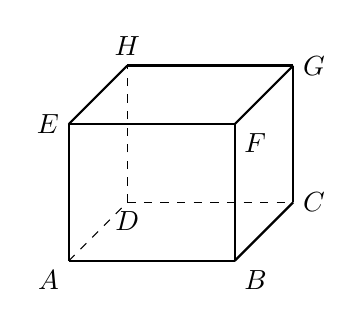
\begin{tikzpicture}[scale=0.62,>=stealth]
\draw[thick] (0,0)--(3.4,0);
\draw[thick] (3.4,0)--(4.6,1.2);
\draw[thick] (4.6,1.2)--(4.6,4.0);
\draw[thick] (0,2.8)--(3.4,2.8);
\draw[thick] (3.4,2.8)--(4.6,4.0);
\draw[thick] (4.6,4.0)--(1.2,4.0);
\draw[thick] (1.2,4.0)--(0,2.8);
\draw[thick] (0,0)--(0,2.8);
\draw[thick] (3.4,0)--(3.4,2.8);
\draw[dashed] (0,0)--(1.2,1.2);
\draw[dashed] (1.2,1.2)--(4.6,1.2);
\draw[dashed] (1.2,1.2)--(1.2,4.0);
\node[below left] at (0,0){$A$};
\node[below right] at (3.4,0){$B$};
\node[right] at (4.6,1.2){$C$};
\node[below] at (1.2,1.2){$D$};
\node[left] at (0,2.8){$E$};
\node[below right] at (3.4,2.8){$F$};
\node[right] at (4.6,4.0){$G$};
\node[above] at (1.2,4.0){$H$};
\end{tikzpicture}
\end{center}
 Bộ ba vectơ nào dưới đây đồng phẳng?}
  {$\overrightarrow{FH}, \overrightarrow{EH}, \overrightarrow{CA}$.}
  {$\overrightarrow{GB}, \overrightarrow{AF}, \overrightarrow{FG}$.}{$\overrightarrow{HF}, \overrightarrow{BG}, \overrightarrow{HG}$.}{$\overrightarrow{BF}, \overrightarrow{CA}, \overrightarrow{BD}$.}


\cauDS[id=C2-B6-D02-TH-052,muc=TH,loigiai={Dùng quy tắc ba điểm và biểu diễn điểm chia, trung điểm, trọng tâm theo các vectơ. a) Đúng. b) Đúng. c) Đúng. d) Sai.}]{Cho hình hộp $EFGH.E'F'G'H'$. Gọi $P$ là điểm thuộc đoạn thẳng $FG$ sao cho $\overrightarrow{FP}=\dfrac{1}{4}\overrightarrow{FG}$. Gọi $J$ là trọng tâm của tam giác $HH'E$. Xét tính đúng sai của các mệnh đề sau:}{%
  \y{$\overrightarrow{FP}=\dfrac{1}{4}\overrightarrow{FG}$.}{d}
  \y{$\overrightarrow{FH}+\overrightarrow{FH'}+\overrightarrow{FE}=3\overrightarrow{FJ}$.}{d}
  \y{$\overrightarrow{JH}+\overrightarrow{JH'}=\overrightarrow{EJ}$.}{d}
  \y{$\overrightarrow{PG}=\dfrac{1}{4}\overrightarrow{FG}$.}{s}}


\cauTLN[id=C2-B6-D02-VD-060,muc=VD,loigiai={Ta có $\overrightarrow{RI}=\dfrac{1}{6}\vec{a}+\vec{b}-\dfrac{2}{3}\vec{c}$ nên $x+y+z=\dfrac{1}{2}$ và $T=6$.}]{Cho hình chóp $S.MNPQ$ có đáy $MNPQ$ là hình bình hành như hình vẽ.
\begin{center}
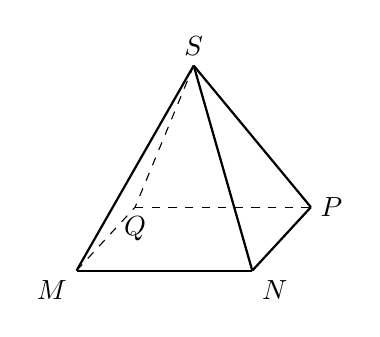
\begin{tikzpicture}[scale=0.62,>=stealth]
\draw[thick] (0,0)--(3.6,0);
\draw[thick] (3.6,0)--(4.8,1.3);
\draw[thick] (2.4,4.2)--(0,0);
\draw[thick] (2.4,4.2)--(3.6,0);
\draw[thick] (2.4,4.2)--(4.8,1.3);
\draw[dashed] (0,0)--(1.2,1.3);
\draw[dashed] (1.2,1.3)--(4.8,1.3);
\draw[dashed] (2.4,4.2)--(1.2,1.3);
\node[below left] at (0,0){$M$};
\node[below right] at (3.6,0){$N$};
\node[right] at (4.8,1.3){$P$};
\node[below] at (1.2,1.3){$Q$};
\node[above] at (2.4,4.2){$S$};
\end{tikzpicture}
\end{center}
Gọi $R$ là điểm thuộc đoạn thẳng $NS$ sao cho $1\overrightarrow{NR}=2\overrightarrow{RS}$. Gọi $I$ là trung điểm của đoạn thẳng $PQ$.  Đặt $\vec{a}=\overrightarrow{MN}$, $\vec{b}=\overrightarrow{MQ}$, $\vec{c}=\overrightarrow{MS}$. Biết $\overrightarrow{RI}=x\vec{a}+y\vec{b}+z\vec{c}$. Tính $T=12(x+y+z)$.}{6}

\cauDS[id=C2-B6-D02-TH-062,muc=TH,loigiai={Dùng quy tắc ba điểm và biểu diễn điểm chia, trung điểm, trọng tâm theo các vectơ. a) Sai. b) Sai. c) Đúng. d) Sai.}]{Cho hình hộp $ABCD.EFGH$ như hình vẽ.
\begin{center}
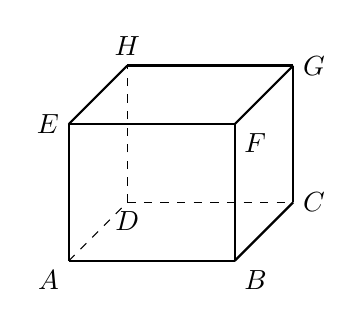
\begin{tikzpicture}[scale=0.62,>=stealth]
\draw[thick] (0,0)--(3.4,0);
\draw[thick] (3.4,0)--(4.6,1.2);
\draw[thick] (4.6,1.2)--(4.6,4.0);
\draw[thick] (0,2.8)--(3.4,2.8);
\draw[thick] (3.4,2.8)--(4.6,4.0);
\draw[thick] (4.6,4.0)--(1.2,4.0);
\draw[thick] (1.2,4.0)--(0,2.8);
\draw[thick] (0,0)--(0,2.8);
\draw[thick] (3.4,0)--(3.4,2.8);
\draw[dashed] (0,0)--(1.2,1.2);
\draw[dashed] (1.2,1.2)--(4.6,1.2);
\draw[dashed] (1.2,1.2)--(1.2,4.0);
\node[below left] at (0,0){$A$};
\node[below right] at (3.4,0){$B$};
\node[right] at (4.6,1.2){$C$};
\node[below] at (1.2,1.2){$D$};
\node[left] at (0,2.8){$E$};
\node[below right] at (3.4,2.8){$F$};
\node[right] at (4.6,4.0){$G$};
\node[above] at (1.2,4.0){$H$};
\end{tikzpicture}
\end{center}
Gọi $P$ là điểm thuộc đoạn thẳng $GF$ sao cho $1\overrightarrow{GP}=3\overrightarrow{PF}$. Gọi $J$ là trọng tâm của tam giác $CAE$.  Xét tính đúng sai của các mệnh đề sau:}{%
  \y{$\overrightarrow{GP}=\dfrac{1}{4}\overrightarrow{GF}$.}{s}
  \y{$\overrightarrow{DC}+\overrightarrow{DA}+\overrightarrow{DE}=\overrightarrow{DJ}$.}{s}
  \y{$\overrightarrow{PF}=\dfrac{1}{4}\overrightarrow{GF}$.}{d}
  \y{$\overrightarrow{AP}=\dfrac{3}{4}\overrightarrow{AG}+\dfrac{1}{4}\overrightarrow{AF}$.}{s}}


\cauTN[id=C2-B6-D02-VD-030,muc=VD,loigiai={Ba vectơ đồng phẳng khi giá của chúng cùng song song với một mặt phẳng, tức là chúng biểu diễn được qua hai vectơ không cùng phương. Với bộ $\overrightarrow{CH}, \overrightarrow{FE}, \overrightarrow{FA}$, ba vectơ cùng nằm trong (hoặc song song với) một mặt phẳng của hình nên đồng phẳng; các bộ còn lại không đồng phẳng.}]{Cho hình hộp $ABCD.EFGH$ như hình vẽ.
\begin{center}
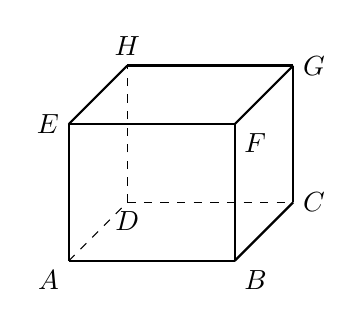
\begin{tikzpicture}[scale=0.62,>=stealth]
\draw[thick] (0,0)--(3.4,0);
\draw[thick] (3.4,0)--(4.6,1.2);
\draw[thick] (4.6,1.2)--(4.6,4.0);
\draw[thick] (0,2.8)--(3.4,2.8);
\draw[thick] (3.4,2.8)--(4.6,4.0);
\draw[thick] (4.6,4.0)--(1.2,4.0);
\draw[thick] (1.2,4.0)--(0,2.8);
\draw[thick] (0,0)--(0,2.8);
\draw[thick] (3.4,0)--(3.4,2.8);
\draw[dashed] (0,0)--(1.2,1.2);
\draw[dashed] (1.2,1.2)--(4.6,1.2);
\draw[dashed] (1.2,1.2)--(1.2,4.0);
\node[below left] at (0,0){$A$};
\node[below right] at (3.4,0){$B$};
\node[right] at (4.6,1.2){$C$};
\node[below] at (1.2,1.2){$D$};
\node[left] at (0,2.8){$E$};
\node[below right] at (3.4,2.8){$F$};
\node[right] at (4.6,4.0){$G$};
\node[above] at (1.2,4.0){$H$};
\end{tikzpicture}
\end{center}
 Bộ ba vectơ nào dưới đây đồng phẳng?}
  {$\overrightarrow{CH}, \overrightarrow{FE}, \overrightarrow{FA}$.}
  {$\overrightarrow{CE}, \overrightarrow{DF}, \overrightarrow{BH}$.}{$\overrightarrow{EA}, \overrightarrow{GB}, \overrightarrow{DB}$.}{$\overrightarrow{ED}, \overrightarrow{AG}, \overrightarrow{FA}$.}


